\documentclass[11pt]{article}

% --- Essential Packages ---
\usepackage[utf8]{inputenc}
\usepackage[margin=1in]{geometry}
\usepackage{amsmath, amssymb} % For thermodynamic equations
\usepackage{graphicx}         % For including your Python plots
\usepackage{booktabs}        % For elegant tables
\usepackage{caption}
\usepackage{subcaption}      % To put plots side-by-side
\usepackage{xurl}
\usepackage[pdftex, hidelinks]{hyperref}
\hypersetup{
    colorlinks=true,
    linkcolor=blue,
    filecolor=magenta,      
    urlcolor=cyan,
}


% --- Document Information ---
\title{ME Grad Assignment 3.2: SOFC Electrochemical Kinetics Fitting}
\author{Ben Rees}
\date{\today}

\begin{document}

\maketitle

\section{Finding Activation Overpotential}

The activation overpotential $\eta_{act} = \eta_{act,O_2}$ is found as the difference between the voltage without the ohmic 
overpotential and the equilibrium voltage, which is given in the problem statement:
$$
\eta_{act} = V_{IR-free} - E \quad\textit{where}\quad V_{IR-free} = V_{meas} - I \cdot R_{ASR},
$$
where all parameters have SI units of Volts, Amperes, and Ohm-meters squared respectively. 

\section{Fitting the Butler-Volmer Equation}
The Butler-Volmer equation is given by:
$$
i = i_0 \left( e^{\frac{\alpha_a F \eta_{A}}{RT}} - e^{-\frac{\alpha_c F \eta_{C}}{RT}} \right)
$$
where $i$ is the current density, $i_0$ is the exchange current density, $\alpha_a$ and $\alpha_c$ are the anodic and cathodic 
charge transfer coefficients, $F$ is Faraday's constant, $R$ is the gas constant, and $T$ is the temperature in Kelvin.

Each of the given data points are compared to the resulting output of the B-V equation given a starting guess for the uknown 
parameters ($i_0$, $\alpha_a$, $\alpha_c$). The sum of squared residuals (SSR) is used as the objective function to minimize:
$$
SSR = \sum_{j=1}^{N} \left( \frac{i_{exp,j} - i_{pred,j}}{1000} \right)^2
$$
where $i_{exp,j}$ is the experimental current density for the $j^{th}$ data point, and $i_{pred,j}$ is the predicted current 
density from the B-V equation. The division by 1000 is used to scale the current densities to kA/m$^2$ for better numerical 
stability during optimization. The optimization is performed using the Sequential Least Squares Programming (SLSQP) method, 
which allows for constraints on the parameters (e.g., $i_0 > 0$, $0 < \alpha_a < 2$, $0 < \alpha_c < 2$). The resulting fit is 
shown in Figure \ref{fig:bv_fit} below:
\begin{figure}[!ht]
    \centering
    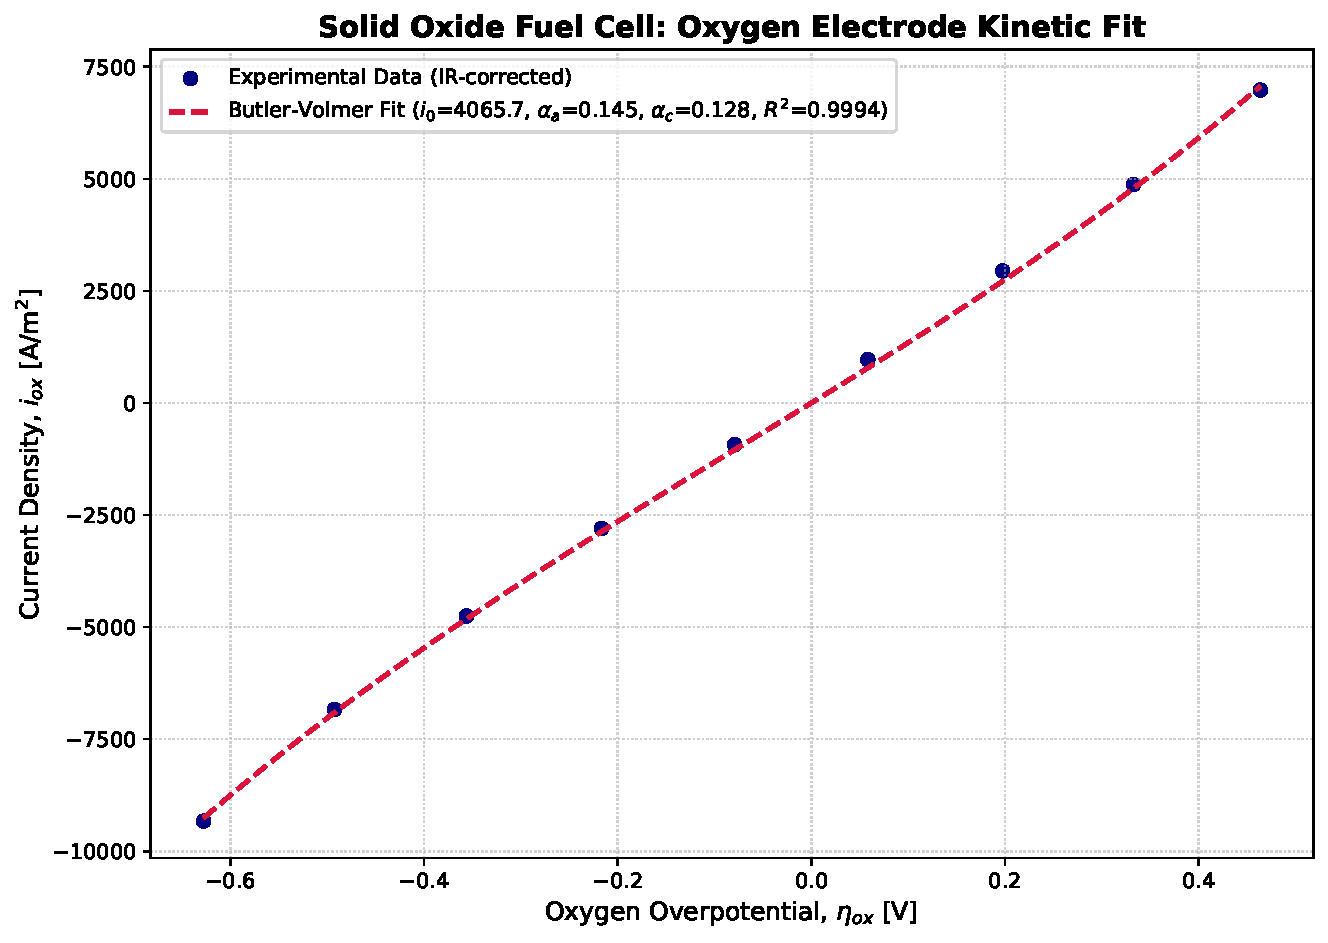
\includegraphics[width=0.8\textwidth]{SOFC_Kinetic_Fit_Results.pdf}
    \caption{Experimental data points (blue circles) and the fitted Butler-Volmer curve (red dashed line) based on the optimized parameters.}
    \label{fig:bv_fit}
\end{figure}
The data is predicted extremely well by the B-V equation, with an $R^2$ value of 0.9994, indicating an excellent fit to the 
experimental data. The most fitting approximation depends on the calculated overpotential, a judgement which typically follows the 
structure:
\begin{gather*}
\text{Linear Approximation: } |\eta| < \frac{RT}{F} \approx 15\text{ mV} \\
\text{Tafel Approximation: } |\eta| > \frac{RT}{F} \ln(10) \approx 100\text{--}120\text{ mV}
\end{gather*}
The overpotentials and applicable approximations for the given data points are summarized in Table \ref{tab:overpotentials} below:
\begin{table}[!ht]
    \centering
    \begin{tabular}{cc}
        \toprule
        $\eta_{ox}$ (V) & Applicable Approximation \\
        \midrule
        0.464 & Tafel \\
        0.333 & Tafel \\
        0.198 & Tafel \\
        0.058 & Neither \\
        -0.079 & Neither \\
        -0.217 & Tafel \\
        -0.356 & Tafel \\
        -0.492 & Tafel \\
        -0.628 & Tafel \\
        \bottomrule
    \end{tabular}
    \caption{Calculated overpotentials and their corresponding applicable approximations.}
    \label{tab:overpotentials}
\end{table}
On the whole, the range of overpotentials in the data set lends itself to the Tafel approximation; this data consists generally of 
overpotentials too large for the linear approximation to be accurate. 

\section{Code Availability}
The code used to scrape the data, calculate the overpotentials, perform the fitting, and generate the plots is available in my 
GitHub repository: \url{https://github.com/Ben-JaminRees/Fuel-Cell-Course-Spring-2026}.

\end{document}